% ============================================================
%  Module 5 — The Marginalist Revolution
%  From Smith to Simulation · University of Edinburgh
% ============================================================
\documentclass[aspectratio=169, 10pt]{beamer}
\usetheme{metropolis}

% --- Edinburgh colours ----------------------------------------
\definecolor{UoERed}{HTML}{7A2318}
\definecolor{UoEGold}{HTML}{B8860B}
\definecolor{CodeBG}{HTML}{F7F3ED}
\definecolor{CodeFrame}{HTML}{D5C9B1}

\setbeamercolor{palette primary}{bg=UoERed, fg=white}
\setbeamercolor{frametitle}{bg=UoERed, fg=white}
\setbeamercolor{title separator}{fg=UoEGold}
\setbeamercolor{progress bar}{fg=UoEGold, bg=UoEGold!20}
\setbeamercolor{alerted text}{fg=UoERed}
\setbeamercolor{block title}{bg=UoERed!15, fg=UoERed}
\setbeamercolor{block body}{bg=UoERed!5}

% --- Packages -------------------------------------------------
\usepackage[T1]{fontenc}
\usepackage{lmodern}
\usepackage{amsmath, amssymb, mathtools}
\usepackage{listings}
\usepackage{graphicx, booktabs}
\usepackage{tikz}
\usetikzlibrary{arrows.meta, positioning, calc, decorations.pathreplacing}
\usepackage{hyperref}
\hypersetup{colorlinks=true, linkcolor=UoERed, urlcolor=UoERed!70!black}
\setbeamertemplate{navigation symbols}{}

\lstset{
  language=Python,
  basicstyle=\ttfamily\scriptsize,
  keywordstyle=\color{UoERed}\bfseries,
  commentstyle=\color{gray}\itshape,
  stringstyle=\color{UoEGold},
  backgroundcolor=\color{CodeBG},
  frame=single,
  rulecolor=\color{CodeFrame},
  numbers=none,
  breaklines=true,
  showstringspaces=false,
  tabsize=4,
  xleftmargin=4pt, xrightmargin=4pt,
  aboveskip=6pt, belowskip=4pt,
}

% Section title pages
\AtBeginSection[]{
  \begin{frame}
    \vfill\centering
    \usebeamerfont{title}\insertsectionhead\par
    \vfill
  \end{frame}
}

% ---- Title ---------------------------------------------------
\title{Module 5 --- The Marginalist Revolution}
\subtitle{Utility, Optimisation, and the Birth of Neoclassical Economics}
\author{Dr Juan Zurita}
\institute{From Smith to Simulation\\
The University of Edinburgh~$\cdot$~School of Economics}
\date{}

\begin{document}

% =============================================================
\maketitle
% =============================================================

% -------------------------------------------------------------
\section{Part I --- The History}
% -------------------------------------------------------------

\begin{frame}{The Revolution of the 1870s}
\begin{columns}[T]
\column{0.55\textwidth}
\begin{itemize}
  \item In the early 1870s, three economists working \textbf{independently}
        arrived at the same idea almost simultaneously.
  \item They called it \alert{marginal utility}, and it transformed economics
        from a study of classes and nations into a science of
        \textbf{individual choice}.
  \item One of the most remarkable cases of simultaneous discovery
        in the history of ideas.
\end{itemize}
\column{0.4\textwidth}
\begin{block}{The Three Founders}
\begin{description}
  \item[Jevons] Manchester, 1871
  \item[Menger] Vienna, 1871
  \item[Walras] Lausanne, 1874
\end{description}
\end{block}
\end{columns}
\end{frame}

\begin{frame}{William Stanley Jevons (1835--1882)}
\begin{columns}[T]
\column{0.55\textwidth}
\begin{itemize}
  \item English economist and logician, professor at Manchester.
  \item \textit{The Theory of Political Economy} (1871):
        economics is ``a calculus of pleasure and pain.''
  \item Used mathematics and the language of \textbf{differential calculus}
        to formalise the idea of diminishing satisfaction.
\end{itemize}
\vspace{0.5em}
\begin{center}
\textit{``Value depends entirely upon utility \ldots\ We have only\\
to trace out carefully the natural laws of the variation\\
of utility.''}\\[4pt]
--- Jevons (1871)
\end{center}
\column{0.4\textwidth}
\begin{block}{Key Idea}
The value of a good is determined not by the total satisfaction
it provides, but by the satisfaction from the \alert{last} unit
consumed --- its \textbf{marginal utility}.
\end{block}
\end{columns}
\end{frame}

\begin{frame}{Menger and Walras}
\begin{columns}[T]
\column{0.48\textwidth}
\begin{block}{Carl Menger (1840--1921)}
  \begin{itemize}
    \item Viennese lawyer turned economist.
    \item \textit{Principles of Economics} (1871).
    \item Emphasised \textbf{subjective value}: goods have value because
          individuals value them, not because of embedded labour.
    \item Founded the \textbf{Austrian School}.
  \end{itemize}
\end{block}
\column{0.48\textwidth}
\begin{block}{L\'{e}on Walras (1834--1910)}
  \begin{itemize}
    \item Professor at Lausanne, Switzerland.
    \item \textit{Elements of Pure Economics} (1874).
    \item Developed \textbf{general equilibrium theory}:
          all markets are interconnected and clear simultaneously.
    \item The most mathematically ambitious of the three.
  \end{itemize}
\end{block}
\end{columns}
\end{frame}

\begin{frame}{The Diamond-Water Paradox}
\begin{block}{The Classical Puzzle}
  Water is \textbf{essential for life} but cheap.
  Diamonds are \textbf{useless} but expensive.\\[4pt]
  If value comes from labour or usefulness, why is water cheap?
\end{block}
\vspace{1em}
The classical economists --- Smith, Ricardo, Marx --- answered with the
\textbf{labour theory of value}: goods are worth the labour required
to produce them. But this never fully resolved the paradox, because
water is \textit{more} useful than diamonds.
\vspace{0.5em}
\begin{center}
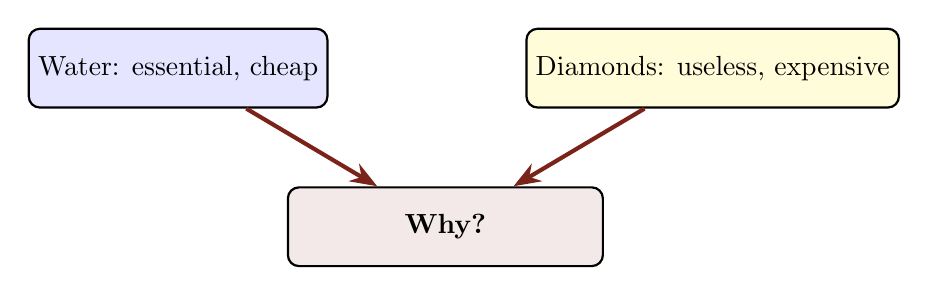
\begin{tikzpicture}[>=Stealth, thick, scale=0.85]
  \node[draw, rounded corners, fill=blue!10, minimum width=3.5cm,
        minimum height=1cm] (water) {Water: essential, cheap};
  \node[right=2.5cm of water, draw, rounded corners, fill=yellow!15,
        minimum width=3.5cm, minimum height=1cm] (diamond) {Diamonds: useless, expensive};
  \node[below=1.5cm of $(water)!0.5!(diamond)$, draw, rounded corners,
        fill=UoERed!10, minimum width=4cm, minimum height=1cm]
        (puzzle) {\textbf{Why?}};
  \draw[->, UoERed, line width=1.5pt] (water) -- (puzzle);
  \draw[->, UoERed, line width=1.5pt] (diamond) -- (puzzle);
\end{tikzpicture}
\end{center}
\end{frame}

\begin{frame}{The Marginalist Answer}
\begin{center}
\textbf{Price reflects \alert{marginal} utility, not \textit{total} utility.}
\end{center}
\vspace{0.5em}
\begin{columns}[T]
\column{0.48\textwidth}
\begin{block}{Water (abundant)}
  \begin{itemize}
    \item Total utility: \textbf{very high}
    \item Marginal utility: \textbf{very low}
    \item The 1000th glass of water adds almost nothing.
  \end{itemize}
\end{block}
\column{0.48\textwidth}
\begin{block}{Diamonds (scarce)}
  \begin{itemize}
    \item Total utility: relatively low
    \item Marginal utility: \textbf{very high}
    \item One more diamond adds a lot.
  \end{itemize}
\end{block}
\end{columns}
\vspace{1em}
It is not the first glass of water vs.\ the first diamond.\\
It is the \textit{last} glass vs.\ the \textit{last} diamond.
\end{frame}

\begin{frame}{What Changed: Three Revolutions in One}
The Marginalist Revolution reshaped economics in three fundamental ways:
\vspace{1em}
\begin{enumerate}
  \item \textbf{From classes to individuals.}\\
        Smith and Marx analysed workers, capitalists, and landlords as classes.
        The marginalists analysed individual consumers and firms making
        \alert{optimising decisions}.
  \vspace{0.5em}
  \item \textbf{From labour theory to subjective value.}\\
        Value became \textbf{subjective} --- determined by individual preferences
        --- rather than objective (embedded labour).
  \vspace{0.5em}
  \item \textbf{Mathematics entered economics.}\\
        Jevons, Walras, and later Marshall expressed economic ideas as
        \textbf{functions, derivatives, and optimisation problems}.
\end{enumerate}
\end{frame}

\begin{frame}{Marshall and the Synthesis}
\begin{columns}[T]
\column{0.55\textwidth}
\begin{itemize}
  \item \textbf{Alfred Marshall} (1842--1924) synthesised the marginalists'
        insights into a coherent framework.
  \item \textit{Principles of Economics} (1890): the standard textbook
        for half a century.
  \item Gave us the \textbf{supply-and-demand diagrams} still used today.
  \item His great achievement: deriving the \alert{demand curve}
        from the theory of consumer choice.
\end{itemize}
\column{0.4\textwidth}
\begin{block}{Marshall's Method}
Put mathematics in the footnotes. Present results with
\textbf{diagrams and intuition}. Let the economics, not the
algebra, be the star.\\[6pt]
\textit{``Burn the mathematics.''}
\end{block}
\end{columns}
\end{frame}

\begin{frame}{Edinburgh Connection}
\begin{block}{The Scottish Tradition}
Edinburgh's intellectual tradition --- with its emphasis on systematic,
evidence-based inquiry going back to the Scottish Enlightenment ---
shaped the reception of marginalism in Britain.
\end{block}
\vspace{0.5em}
\begin{itemize}
  \item Marshall acknowledged debts to the \textbf{Scottish philosophical
        tradition} and its empirical method.
  \item Edinburgh's economics department adopted the new mathematical
        methods \textbf{earlier than many British universities}.
  \item The marginalists' insistence on \textbf{observation and formal reasoning}
        echoed the values of Hume, Smith, and the Enlightenment.
\end{itemize}
\vspace{0.5em}
From Smith's verbal reasoning about the invisible hand to Jevons's
``calculus of pleasure and pain'' --- the Scottish tradition of rigour
endures.
\end{frame}

% -------------------------------------------------------------
\section{Part II --- The Computation}
% -------------------------------------------------------------

\begin{frame}[fragile]{Setting Up}
\begin{lstlisting}
import numpy as np
import matplotlib.pyplot as plt
from scipy.optimize import minimize
\end{lstlisting}
\vspace{0.5em}
\begin{itemize}
  \item \texttt{numpy} --- numerical arrays and operations
  \item \texttt{matplotlib} --- plotting
  \item \texttt{minimize} --- constrained optimisation\\
        (the computational equivalent of choosing the best affordable bundle)
\end{itemize}
\end{frame}

\begin{frame}{Utility and Diminishing Marginal Utility}
A consumer gets satisfaction --- \textbf{utility} --- from consuming goods.
The key insight of the marginalists:
\vspace{0.3em}
\begin{center}
\textit{Utility increases with consumption but at a \alert{decreasing rate}.}
\end{center}
\vspace{0.3em}
A common utility function:
\[
  u(x) = x^{0.5}
\]
The \textbf{marginal utility} is the derivative:
\[
  u'(x) = 0.5 \cdot x^{-0.5}
\]
\vspace{0.3em}
\begin{itemize}
  \item $u'(x) > 0$: more is always better
  \item $u''(x) < 0$: but each additional unit adds less than the one before
  \item This is Jevons's \textbf{law of diminishing marginal utility}
\end{itemize}
\end{frame}

\begin{frame}{Total vs.\ Marginal Utility}
\begin{center}
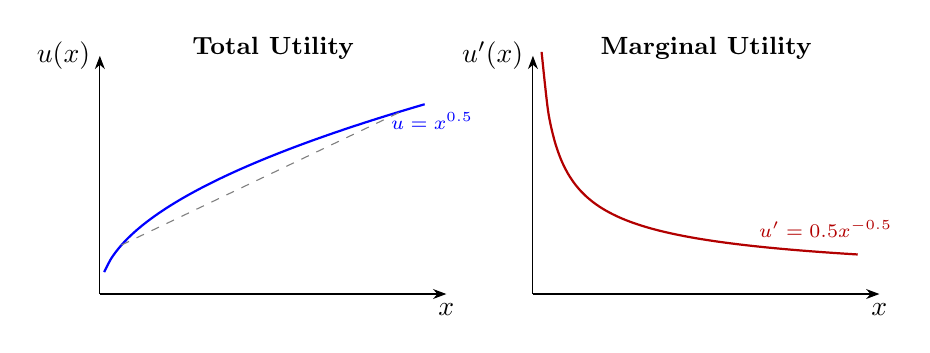
\begin{tikzpicture}[scale=0.55, >=Stealth]
  % --- Total utility plot ---
  \begin{scope}[shift={(0,0)}]
    \draw[->] (0,0) -- (8,0) node[below] {$x$};
    \draw[->] (0,0) -- (0,5.5) node[left] {$u(x)$};
    \draw[thick, blue] plot[smooth, domain=0.1:7.5, samples=50]
      (\x, {1.6*sqrt(\x)});
    \node[above, font=\small\bfseries] at (4, 5.2) {Total Utility};
    \node[right, font=\scriptsize, blue] at (6.5, 4) {$u = x^{0.5}$};
    % Concavity annotation
    \draw[dashed, gray] (0.5, {1.6*sqrt(0.5)}) -- (7, {1.6*sqrt(7)});
  \end{scope}
  % --- Marginal utility plot ---
  \begin{scope}[shift={(10,0)}]
    \draw[->] (0,0) -- (8,0) node[below] {$x$};
    \draw[->] (0,0) -- (0,5.5) node[left] {$u'(x)$};
    \draw[thick, red!70!black] plot[smooth, domain=0.2:7.5, samples=50]
      (\x, {2.5/sqrt(\x)});
    \node[above, font=\small\bfseries] at (4, 5.2) {Marginal Utility};
    \node[right, font=\scriptsize, red!70!black] at (5, 1.5) {$u' = 0.5x^{-0.5}$};
  \end{scope}
\end{tikzpicture}
\end{center}
\vspace{0.3em}
The first slice of cake is heavenly; the tenth is merely okay;
the twentieth might make you ill.
\end{frame}

\begin{frame}[fragile]{Plotting Utility in Python}
\begin{lstlisting}
x = np.linspace(0.01, 10, 200)

fig, axes = plt.subplots(1, 2, figsize=(12, 4.5))

# Total utility
axes[0].plot(x, x**0.5, color='steelblue', linewidth=2.5)
axes[0].set_xlabel('Quantity consumed')
axes[0].set_ylabel('Utility u(x)')
axes[0].set_title('Total Utility: Increasing but Concave')

# Marginal utility
axes[1].plot(x, 0.5 * x**(-0.5), color='coral', linewidth=2.5)
axes[1].set_xlabel('Quantity consumed')
axes[1].set_ylabel("Marginal utility u'(x)")
axes[1].set_title('Marginal Utility: Positive but Falling')

plt.tight_layout()
plt.show()
\end{lstlisting}
\end{frame}

\begin{frame}[fragile]{The Diamond-Water Paradox: A Numerical Example}
\begin{lstlisting}
# u(x) = x^0.5
water_quantity = 100    # abundant
diamond_quantity = 0.5  # scarce

total_u_water = water_quantity**0.5          # 10.00
marginal_u_water = 0.5 * water_quantity**(-0.5)    # 0.05

total_u_diamond = diamond_quantity**0.5      #  0.71
marginal_u_diamond = 0.5 * diamond_quantity**(-0.5) # 0.71
\end{lstlisting}
\vspace{0.3em}
\begin{center}
\begin{tabular}{lcc}
\toprule
 & Water ($x=100$) & Diamonds ($x=0.5$) \\
\midrule
Total utility    & $10.00$ \textbf{(high)} & $0.71$ \\
Marginal utility & $0.05$                  & $0.71$ \textbf{(high)} \\
\bottomrule
\end{tabular}
\end{center}
\vspace{0.5em}
Price reflects \alert{marginal utility}, not total utility.\\
That is why diamonds cost more than water.
\end{frame}

\begin{frame}{Consumer Choice: Two Goods and a Budget}
The marginalists' core problem:
\vspace{0.3em}
\[
  \max_{x_1, x_2}\; u(x_1, x_2) \quad \text{subject to} \quad
  p_1 x_1 + p_2 x_2 \leq m
\]
\vspace{0.3em}
We use the \textbf{Cobb-Douglas utility function}:
\[
  u(x_1, x_2) = x_1^a \cdot x_2^{1-a}
\]
\vspace{0.3em}
\begin{itemize}
  \item $a$ governs how much the consumer values good~1 vs.\ good~2.
  \item Parameters: $a = 0.4$, $p_1 = 2$, $p_2 = 3$, $m = 120$.
\end{itemize}
\vspace{0.5em}
\begin{block}{Analytical Solution (Cobb-Douglas)}
\[
  x_1^* = \frac{a \cdot m}{p_1} = \frac{0.4 \times 120}{2} = 24, \qquad
  x_2^* = \frac{(1-a) \cdot m}{p_2} = \frac{0.6 \times 120}{3} = 24
\]
\end{block}
\end{frame}

\begin{frame}{Indifference Curves and the Budget Line}
\begin{center}
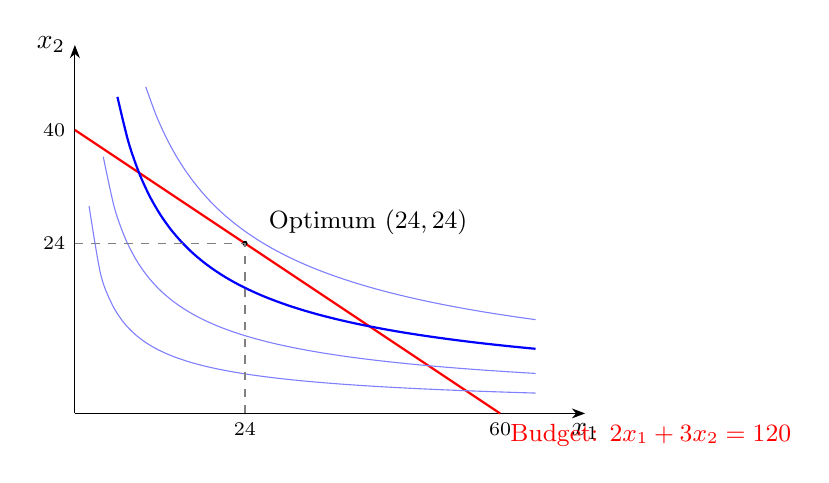
\begin{tikzpicture}[scale=0.09, >=Stealth]
  % Axes
  \draw[->] (0,0) -- (72,0) node[below] {$x_1$};
  \draw[->] (0,0) -- (0,52) node[left] {$x_2$};
  % Budget line: x2 = (120 - 2*x1)/3 = 40 - (2/3)*x1
  \draw[thick, red] (0,40) -- (60,0)
    node[below right, font=\small] {Budget: $2x_1 + 3x_2 = 120$};
  % Indifference curves: x2 = (u / x1^0.4)^(1/0.6)
  % u=10: x2 = (10/x1^0.4)^(1.667)
  \draw[thin, blue!50] plot[smooth, domain=2:65, samples=40]
    (\x, {(10/(\x^0.4))^1.667});
  % u=15
  \draw[thin, blue!50] plot[smooth, domain=4:65, samples=40]
    (\x, {(15/(\x^0.4))^1.667});
  % u=20 (optimal ~ this level)
  \draw[thick, blue] plot[smooth, domain=6:65, samples=40]
    (\x, {(20/(\x^0.4))^1.667});
  % u=25
  \draw[thin, blue!50] plot[smooth, domain=10:65, samples=40]
    (\x, {(25/(\x^0.4))^1.667});
  % Optimal point (24, 24)
  \filldraw[black] (24, 24) circle (8pt);
  \draw[dashed, gray] (24, 0) -- (24, 24) -- (0, 24);
  \node[right, font=\small] at (26, 27) {Optimum $(24, 24)$};
  \node[below, font=\scriptsize] at (24, 0) {$24$};
  \node[left, font=\scriptsize] at (0, 24) {$24$};
  % Axis labels
  \node[below, font=\scriptsize] at (60, 0) {$60$};
  \node[left, font=\scriptsize] at (0, 40) {$40$};
\end{tikzpicture}
\end{center}
\vspace{0.3em}
The consumer reaches the \textbf{highest indifference curve}
that still touches the budget constraint --- the tangency point.
\end{frame}

\begin{frame}{The Tangency Condition}
At the optimum, the slope of the indifference curve equals the slope of the
budget line:
\[
  \underbrace{\frac{MU_1}{MU_2}}_{\text{Marginal rate of substitution}}
  = \underbrace{\frac{p_1}{p_2}}_{\text{Price ratio}}
\]
\vspace{0.3em}
\begin{itemize}
  \item \textbf{MRS} $= \dfrac{a}{1-a}\cdot\dfrac{x_2}{x_1}$
        for Cobb-Douglas.
  \item At the optimum: $\dfrac{0.4}{0.6}\cdot\dfrac{24}{24}
        = \dfrac{2}{3} = \dfrac{p_1}{p_2}$ \checkmark
  \item Intuition: the rate at which the consumer is \textit{willing}
        to trade goods equals the rate at which the market \textit{allows} it.
\end{itemize}
\end{frame}

\begin{frame}[fragile]{Solving with \texttt{scipy.optimize.minimize}}
Since \texttt{minimize} minimises, we minimise \textbf{negative} utility:
\begin{lstlisting}
a, p1, p2, m = 0.4, 2, 3, 120

def neg_utility(x):
    x1, x2 = x
    if x1 <= 0 or x2 <= 0:
        return 1e10  # penalty for non-positive consumption
    return -(x1**a * x2**(1 - a))

budget = {'type': 'ineq',
          'fun': lambda x: m - p1*x[0] - p2*x[1]}
bounds = [(0.01, None), (0.01, None)]

result = minimize(neg_utility, x0=[10, 10],
                  method='SLSQP',
                  bounds=bounds, constraints=budget)

x1_star, x2_star = result.x
print(f"x1* = {x1_star:.2f}, x2* = {x2_star:.2f}")
# x1* = 24.00, x2* = 24.00
\end{lstlisting}
\end{frame}

\begin{frame}[fragile]{Verifying the Solution}
\begin{lstlisting}
u_star = x1_star**a * x2_star**(1 - a)

print(f"Optimal bundle:")
print(f"  x1* = {x1_star:.2f} (spending {p1*x1_star:.0f})")
print(f"  x2* = {x2_star:.2f} (spending {p2*x2_star:.0f})")
print(f"  Total spending: {p1*x1_star + p2*x2_star:.0f}")
print(f"  Utility: {u_star:.4f}")

# Analytical solution for Cobb-Douglas
x1_a = a * m / p1      # = 24
x2_a = (1-a) * m / p2  # = 24
print(f"\nAnalytical: x1* = {x1_a}, x2* = {x2_a}")
\end{lstlisting}
\vspace{0.5em}
\begin{block}{Cobb-Douglas Property}
The consumer spends exactly fraction $a$ of income on good~1
and $(1-a)$ on good~2, \textbf{regardless of prices}.
\[
  p_1 x_1^* = a \cdot m = 0.4 \times 120 = 48, \qquad
  p_2 x_2^* = (1-a) \cdot m = 0.6 \times 120 = 72
\]
\end{block}
\end{frame}

\begin{frame}[fragile]{Deriving the Demand Curve}
Marshall's great achievement: deriving the demand curve from consumer choice.\\
As $p_1$ rises, the consumer buys less of good~1.
\begin{lstlisting}
p1_range = np.linspace(0.5, 10, 30)
x1_demand = []

for p1_val in p1_range:
    cons = {'type': 'ineq',
            'fun': lambda x, p=p1_val: m - p*x[0] - p2*x[1]}
    res = minimize(neg_utility, x0=[10, 10], method='SLSQP',
                   bounds=[(0.01, None), (0.01, None)],
                   constraints=cons)
    x1_demand.append(res.x[0])

# Analytical demand: x1* = a*m/p1
x1_analytical = a * m / p1_range
\end{lstlisting}
\vspace{0.3em}
The demand curve slopes downward --- exactly as Marshall drew it in 1890.\\
But now we have \textbf{derived} it from individual optimisation, not assumed it.
\end{frame}

\begin{frame}{The Demand Curve}
\begin{center}
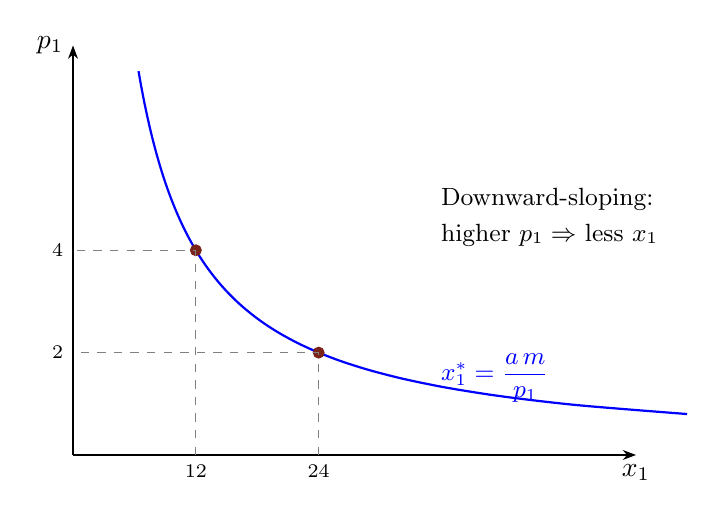
\begin{tikzpicture}[scale=0.65, >=Stealth]
  % Axes
  \draw[->] (0,0) -- (11,0) node[below] {$x_1$};
  \draw[->] (0,0) -- (0,8) node[left] {$p_1$};
  % Demand curve: x1 = a*m/p1 = 48/p1
  % At p1=1, x1=48; at p1=2, x1=24; at p1=4, x1=12; at p1=8, x1=6; at p1=10, x1=4.8
  % Scale: x1/5 for x-axis, p1 for y-axis
  \draw[thick, blue] plot[smooth, domain=0.8:7.5, samples=40]
    ({48/(5*\x)}, \x);
  \node[right, font=\small, blue] at (7, 1.5) {$x_1^* = \dfrac{a\,m}{p_1}$};
  % Points
  \filldraw[UoERed] ({48/10}, 2) circle (3pt);
  \draw[dashed, gray] ({48/10}, 0) -- ({48/10}, 2) -- (0, 2);
  \node[below, font=\scriptsize] at ({48/10}, 0) {$24$};
  \node[left, font=\scriptsize] at (0, 2) {$2$};
  \filldraw[UoERed] ({48/20}, 4) circle (3pt);
  \draw[dashed, gray] ({48/20}, 0) -- ({48/20}, 4) -- (0, 4);
  \node[below, font=\scriptsize] at ({48/20}, 0) {$12$};
  \node[left, font=\scriptsize] at (0, 4) {$4$};
  % Annotation
  \node[right, font=\small] at (7, 5) {Downward-sloping:};
  \node[right, font=\small] at (7, 4.3) {higher $p_1 \Rightarrow$ less $x_1$};
\end{tikzpicture}
\end{center}
\vspace{0.3em}
A higher $p_1$ has both an \textbf{income effect} (consumer is poorer)
and a \textbf{substitution effect} (good~1 is relatively more expensive),
both reducing demand for a normal good.
\end{frame}

\begin{frame}{From Utility to Markets: The Big Picture}
\begin{center}
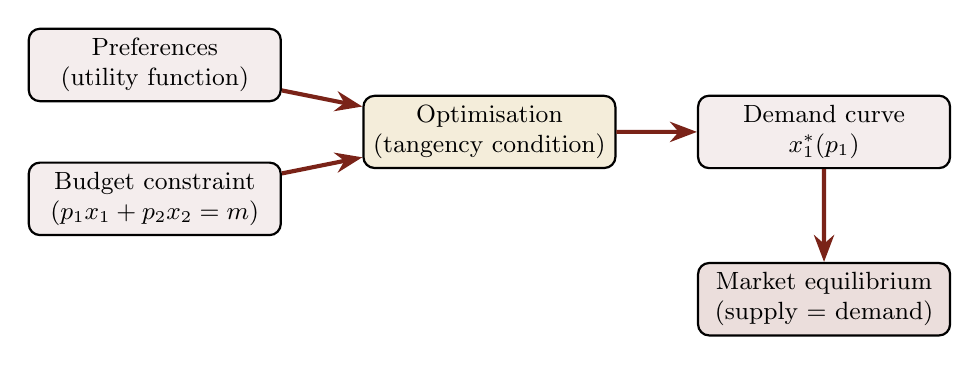
\begin{tikzpicture}[>=Stealth, thick, scale=0.85,
  box/.style={draw, rounded corners, fill=UoERed!8,
              minimum width=3.2cm, minimum height=0.9cm,
              font=\small, align=center}]
  \node[box] (pref) at (0, 4) {Preferences\\(utility function)};
  \node[box] (budget) at (0, 2) {Budget constraint\\($p_1 x_1 + p_2 x_2 = m$)};
  \node[box, fill=UoEGold!15] (opt) at (5, 3) {Optimisation\\(tangency condition)};
  \node[box] (demand) at (10, 3) {Demand curve\\$x_1^*(p_1)$};
  \node[box, fill=UoERed!15] (mkt) at (10, 0.5) {Market equilibrium\\(supply = demand)};
  \draw[->, line width=1.5pt, UoERed] (pref) -- (opt);
  \draw[->, line width=1.5pt, UoERed] (budget) -- (opt);
  \draw[->, line width=1.5pt, UoERed] (opt) -- (demand);
  \draw[->, line width=1.5pt, UoERed] (demand) -- (mkt);
\end{tikzpicture}
\end{center}
\vspace{0.5em}
The marginalists provided \alert{microfoundations} for Smith's supply-and-demand model:
individual rational choice generates the demand curve, which then determines
market equilibrium.
\end{frame}

% -------------------------------------------------------------
\section{Part III --- Exercises \& Discussion}
% -------------------------------------------------------------

\begin{frame}{Exercise 1: Income and Substitution Effects}
When the price of good~1 rises, two things happen:
\vspace{0.3em}
\begin{enumerate}
  \item The consumer is effectively \textbf{poorer} (income effect).
  \item Good~1 is now \textbf{relatively more expensive} (substitution effect).
\end{enumerate}
\vspace{0.5em}
Using $a = 0.4$, $p_2 = 3$, $m = 120$:
\vspace{0.3em}
\begin{enumerate}[(a)]
  \item Compute $x_1^*$ at $p_1 = 2$ and at $p_1 = 4$. What is $\Delta x_1$?
  \item \textbf{Compensated demand:} at $p_1 = 4$, how much income would keep
        utility at the old level? Use \texttt{minimize} to find the minimum
        expenditure that achieves $u^*_{\text{old}}$.
  \item Compute the substitution effect and income effect separately.
        Verify they sum to $\Delta x_1$.
  \item For a \textbf{normal good}, both effects reduce $x_1$. Verify.
\end{enumerate}
\end{frame}

\begin{frame}{Exercise 2: Beyond Cobb-Douglas --- CES Utility}
The \textbf{CES} utility function allows different degrees of substitutability:
\[
  u(x_1, x_2) = \bigl( a \cdot x_1^\rho + (1-a) \cdot x_2^\rho \bigr)^{1/\rho}
\]
where $\rho = (\sigma - 1)/\sigma$ and $\sigma$ is the elasticity of substitution.
\vspace{0.5em}
\begin{enumerate}[(a)]
  \item Define a CES utility function. Using $a = 0.5$, $p_1 = 2$, $p_2 = 3$,
        $m = 120$, solve for $\sigma = 0.5, 1, 2, 5$.
  \item Derive the demand curve for each $\sigma$ (vary $p_1$ from 0.5 to 8).
        Plot all four on one graph. Which $\sigma$ gives the most elastic demand?
  \item What happens as $\sigma \to \infty$? (Hint: perfect substitutes.)
        What does the demand curve look like?
\end{enumerate}
\end{frame}

\begin{frame}{Exercise 3: From Smith to the Marginalists}
In Module~1 we found market equilibrium by setting supply equal to demand.
Now we can \textit{derive} the demand curve from first principles.
\vspace{0.5em}
\begin{enumerate}[(a)]
  \item 100 identical consumers each have $m = 120$ and Cobb-Douglas utility
        with $a = 0.4$. Compute the \textbf{aggregate demand curve}:
        total demand $= 100 \times x_1^*(p_1)$.
  \item Define a linear supply: $Q^S(p_1) = 500 + 200\,p_1$.
  \item Use \texttt{fsolve} to find the market equilibrium.
        Plot supply and demand.
  \item In 2--3 sentences, explain how the marginalist approach provides
        \alert{microfoundations} for the supply-and-demand model
        Smith described verbally.
\end{enumerate}
\end{frame}

% -------------------------------------------------------------
\section{Quiz}
% -------------------------------------------------------------

\begin{frame}{Quiz: Conceptual Questions}
\begin{enumerate}
  \item The diamond-water paradox is resolved by recognising that price reflects:\\
        (a) Total utility \quad (b) \alert{Marginal utility} \quad
        (c) Labour content \quad (d) Production cost
  \vspace{0.3em}
  \item The Marginalist Revolution shifted economics from:\\
        (a) Trade to monetary theory \quad
        (b) \alert{Class-based analysis to individual optimisation}\\
        (c) Mathematics to verbal reasoning \quad
        (d) Micro to macroeconomics
  \vspace{0.3em}
  \item Diminishing marginal utility means:\\
        (a) Total utility decreases \\
        (b) \alert{Each additional unit provides less additional satisfaction}\\
        (c) Utility is negative beyond some point \quad
        (d) Consumers prefer less to more
  \vspace{0.3em}
  \item Marshall's main contribution was:\\
        (a) Inventing calculus\\
        (b) \alert{Synthesising marginalist theory into supply-and-demand}\\
        (c) Disproving comparative advantage \quad
        (d) Founding the LSE
\end{enumerate}
\end{frame}

\begin{frame}{Quiz: Computational Questions}
\begin{enumerate}\setcounter{enumi}{4}
  \item The consumer's optimal bundle is where:\\
        (a) All income goes to the cheaper good\\
        (b) \alert{The highest indifference curve touches the budget constraint}\\
        (c) Marginal utility is zero \quad
        (d) Budget constraint crosses the origin
  \vspace{0.3em}
  \item For $u = x_1^{0.4}x_2^{0.6}$ with $p_1=2$, $p_2=3$, $m=120$,
        the optimal $x_1^*$ is:\\
        (a) \alert{$0.4 \times 120/2 = 24$} \quad (b) $36$ \quad
        (c) $60$ \quad (d) $16$
  \vspace{0.3em}
  \item To maximise utility using \texttt{minimize}, we minimise:\\
        (a) Utility directly \quad (b) \alert{Negative utility} \quad
        (c) The budget constraint \quad (d) Price times quantity
  \vspace{0.3em}
  \item For Cobb-Douglas utility, the share of income spent on good~1 is:\\
        (a) Always 50\% \quad (b) \alert{Equal to the exponent $a$} \quad
        (c) Depends on the price ratio \quad (d) $1$ minus the price ratio
\end{enumerate}
\end{frame}

% -------------------------------------------------------------
\section{Key Takeaways}
% -------------------------------------------------------------

\begin{frame}{What We Learned This Week}
\begin{enumerate}
  \item The \textbf{Marginalist Revolution} (1870s) shifted economics from
        class-based, labour-theory reasoning to \textbf{individual optimisation}
        with subjective value.
  \item The \textbf{diamond-water paradox} dissolves once we distinguish
        \textit{total} from \textit{marginal} utility.
  \item Consumers maximise utility subject to a \textbf{budget constraint};
        the solution is the tangency between the highest indifference curve
        and the budget line.
  \item \texttt{scipy.optimize.minimize} with \texttt{SLSQP} solves
        constrained optimisation problems --- minimise negative utility.
  \item The \textbf{demand curve} can be \textit{derived} from utility
        maximisation, not just assumed --- providing \alert{microfoundations}
        for Smith's supply-and-demand intuition.
\end{enumerate}
\end{frame}

\begin{frame}{Further Reading}
\begin{itemize}
  \item Jevons, W.S.\ \textit{The Theory of Political Economy} (1871), Ch.~3.
  \item Backhouse, R.\ \textit{The Penguin History of Economics}, Ch.~7\\
        (``The Marginalist Revolution'').
  \item Marshall, A.\ \textit{Principles of Economics} (1890), Book~III\\
        (on demand and utility).
  \item Mas-Colell, A., Whinston, M., \& Green, J.\ \textit{Microeconomic Theory},
        Ch.~3 (for the mathematically adventurous).
\end{itemize}
\vspace{1em}
\begin{center}
\textbf{Next week:} Keynes and the Great Depression ---\\
why the marginalists' beautiful model of rational individuals\\
could not explain mass unemployment.
\end{center}
\end{frame}

\end{document}
